\section{Variationen}
Es gibt verschiedenste Variationen des Downhill-Simplex Algorithmus.
Einige verwenden zusätzliche Freiheitsgrade, wie z.B. einen Parameter
$\sigma$, welcher $\beta$ bei Komprimierung ersetzt.

Auch gibt es Erweiterungen welche statistische Auswertung bei verrauschten Zielfunktionen (siehe \figref{fig:downhillRauschen1}) durchführen.
Verrauschte Zielfunktionen treten unter anderem auf wenn man Parameter f"ur ein System optimieren will, welche sich nur durch Messung vergleichen lassen.
Obwohl auch der ''normale`` Downhill-Simplex mehr oder weniger funktioniert (siehe \figref{fig:downhillRauschen2}), hat er m"uhe zu konvergieren, da er immer auch die Chance hat sich fälschlicherweise auszudehnen.
Wie man sieht ist viel Potential vorhanden indem der Einfluss des Rauschens verringert wird.
Informationen dazu unter \footnote{\url{http://www.informs-sim.org/wsc91papers/1991_0126.pdf}}
\begin{figure}[h]
\centering
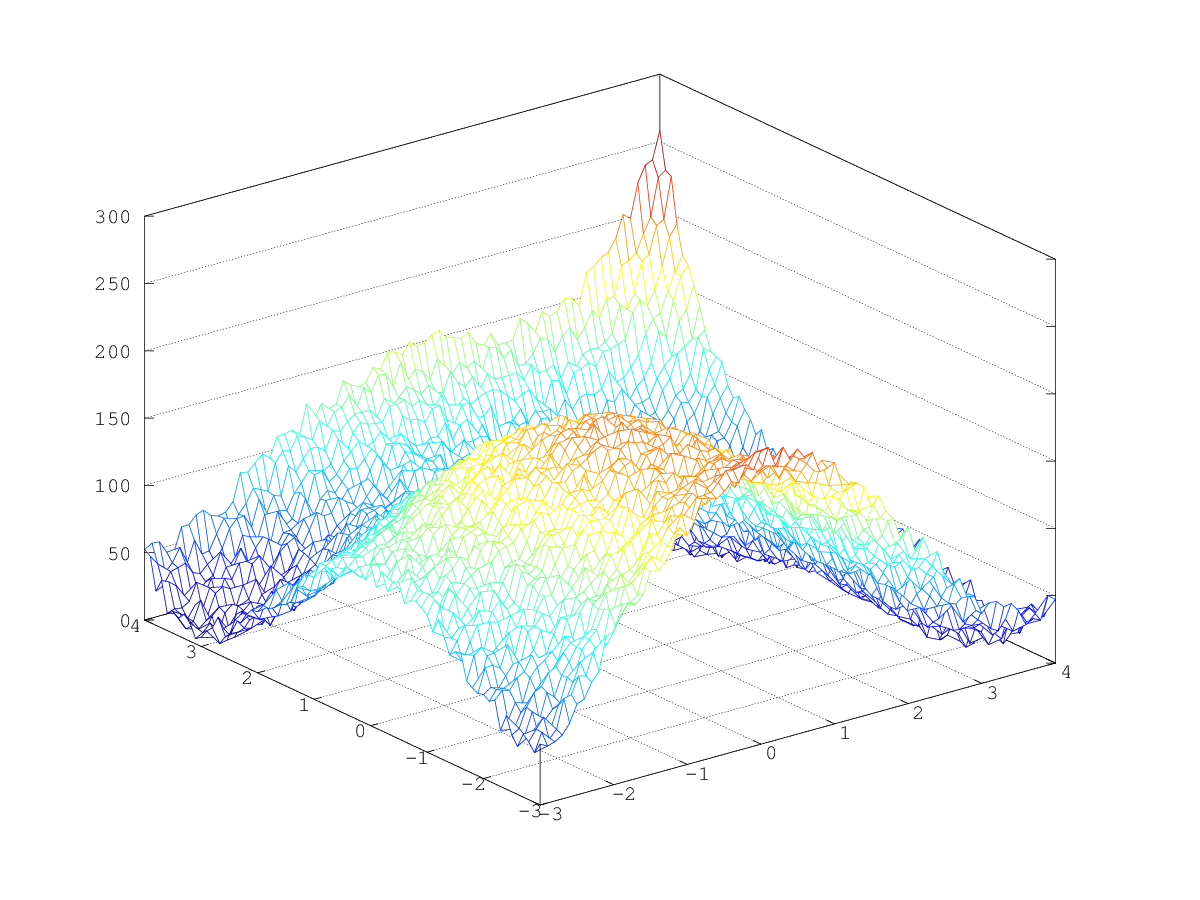
\includegraphics[width=0.8\textwidth]{../bilder/HimmelblauRandom/himmelblauoverview.png}
\caption{Verrauschte Zielfunktion}
\label{fig:downhillRauschen1}
\end{figure}

\begin{figure}[h]
\centering
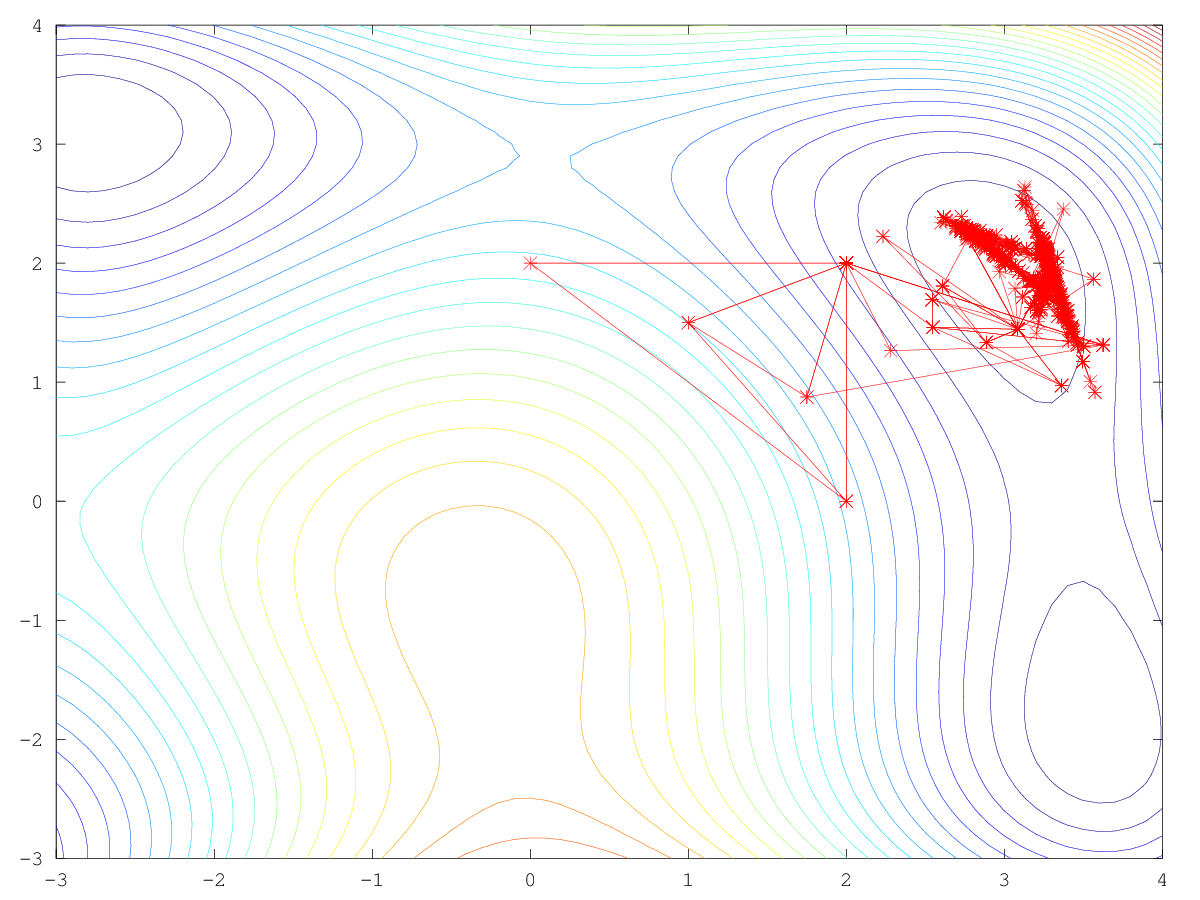
\includegraphics[width=0.8\textwidth]{../bilder/HimmelblauRandom/himmelblauall.png}
\caption{Beispiel Verlauf Simplex mit verrauschter Zielfunktion}
\label{fig:downhillRauschen2}
\end{figure}